\documentclass[12pt]{report}

% Import packages
\usepackage{listings}  % For adding C++ code
\usepackage{xcolor}    % For custom colors
\usepackage{graphicx}  % For including images
\usepackage{hyperref}  % For creating hyperlinks
\usepackage{geometry}  % To set page margins
\usepackage{subfig}
\geometry{a4paper, margin=1in}
\begin{document}

\lstdefinestyle{javastyle}{
    language=Java,
    basicstyle=\ttfamily\footnotesize, % Font style
    keywordstyle=\color{purple}\bfseries, % Keywords in blue
    stringstyle=\color{orange}, % Strings in red
    commentstyle=\color{olive}, % Comments in gray
    numbers=none, % No line numbers
    tabsize=4, % Tab space width
    showspaces=false,
    showstringspaces=false,
    frame=single, % Adds a single-line box around the code
    framerule=0.8pt, % Thickness of the frame
    framesep=5pt, % Space between frame and code
}

\title{\textbf{Computer Networks 2 - Chat App}}
\author{Tzanetis Savvas, Zoidis Vasilis}
\maketitle  % Creates the title

\tableofcontents  % Generates the table of contents
\newpage

\chapter{Introduction}

This report is part of an assignment for the \textbf{Computer Networks 2} class for the \textbf{Electrical and Computer Engineering} department of the \textbf{Aristotle University of Thessaloniki}. The objective of the assignment is to create a \textbf{Peer-to-Peer} Chat and VoIP application using the \textbf{Java} programming language and its included libraries without relying on external dependencies. Communication will be achieved using the \textbf{UDP Protocol} with the \textbf{java.net} library.

The code for this assignment can be found at \href{https://github.com/stzanetis/p2p-chatapp}{this GitHub page}.

\chapter{Code Implementations}
\section{Text Encryption}
This implementation uses internal java libraries in order to encrypt/decrypt the text messages that are being sent through the application. This is a very important step since if the packages that contain the text messages are not encrypted, their contents will be visible to anyone currently connected to any of the sender or receiver networks, something that can be observed using \textbf{Wireshark} and that we will show later in the report. In order to encrypt and decrypt such packages, a shared secret key is needed between the two connected clients. For the purposes of this implementation a static pre-shared key is used, but it is highly recommended to have secret keys exchanged using methods like the \textbf{Diffie-Hellman} or \textbf{Double Ratchet Algorithm} methods.

The code below shows the function handling the encryption and decryption process for the text messages:
\begin{lstlisting}[style=javastyle]
private static String encryptMessage(String message) {
	try {
		Cipher cipher = Cipher.getInstance("AES");
		cipher.init(Cipher.ENCRYPT_MODE, secretKey);
		byte[] encrypted = cipher.doFinal(message.getBytes());
		return Base64.getEncoder().encodeToString(encrypted);
	} catch (Exception e) {
		e.printStackTrace();
		return null;
	}
}

private static String decryptMessage(String message) {
	try {
		Cipher cipher = Cipher.getInstance("AES");
		cipher.init(Cipher.DECRYPT_MODE, secretKey);
		byte[] decrypted = cipher.doFinal(
                           Base64.getDecoder().decode(message));
		return new String(decrypted);
	} catch (Exception e) {
		e.printStackTrace();
		System.out.println("Error Decrypting");
		return null;
	}
}
\end{lstlisting}

\section{Sending and Receiving Text messages}
Text messages are being sent using the UDP protocol. A dedicated thread is created to listen for incoming messages from a specific IP (in case multiple communications are made using the same network). The port used to send and receive these messages is \textbf{Port 12345} as specified in the assignment instructions. \\
Below, is the snippet demonstrating the implementation for the listening thread used for receiving any text messages:
\begin{lstlisting}[style=javastyle]
new Thread(() -> {
	byte[] buffer = new byte[1024];
	try (
         DatagramSocket textSocket = new DatagramSocket(
                                         Integer.parseInt(chatPort)))
    {
		while (true) {
			DatagramPacket packet = new DatagramPacket(
                                        buffer, buffer.length);
			textSocket.receive(packet);
			if (packet.getAddress().getHostAddress().equals(destIp))
            {
				String message = new String(
                                    packet.getData(), 0, 
                                    packet.getLength());
				textArea.append(
                    "Received: " + decryptMessage(message) + newline);
			}
		}
	} catch (IOException e) {
		e.printStackTrace();
	}
}).start();
\end{lstlisting}
\vfill
The image below, shows a \textbf{Wireshark} window, verifying that the text packages are being sent on \textbf{Port 12345}. The two IPs used are local IPs since it is a local connection between two computers, with the right firewall and network configurations for port forwarding, a connection between multiple networks is also possible.
\begin{figure}[h!]
    \centering
    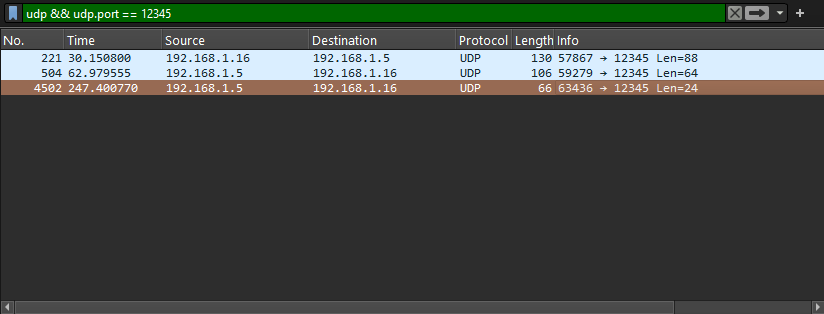
\includegraphics[width=1\linewidth]{Screenshot 2024-12-12 112931.png}
    \caption{Package streams for text messages}
    \label{fig:enter-label}
\end{figure}
\newpage
The following code snippet is run only when the "Send" button is pressed by the user, a packet with the message is being sent to the receiver only if the string inside the text field is not empty (only if an actual message has been written).
\begin{lstlisting}[style=javastyle]
// The "Send" button was clicked
String message = inputTextField.getText();
if (!message.trim().isEmpty()) {
	try {
		DatagramSocket textSocket = new DatagramSocket();
		InetAddress address = InetAddress.getByName(destIp);
		int port = Integer.parseInt(chatPort);
		byte[] buffer = encryptMessage(message).getBytes();
		DatagramPacket packet = new DatagramPacket(
                                    buffer, buffer.length, 
                                    address, port);

		// Print the message locally
		textArea.append("Me: " + message + newline);
		inputTextField.setText("");

		//Send the message to the target
		textSocket.send(packet);
		textSocket.close();
		System.out.println("Message sent");
	} catch (IOException ex) {
		ex.printStackTrace();
	}
}
\end{lstlisting}
\vfill
The image below, shows the contents from an individual package, revealing its Network headers, as well as its encrypted payload (also in hexadecimal form). If we decrypted the string showed using the encryption key used ("abcdefghigklmnop") based on the \textbf{Advanced Encryption Standard}, the final message would be \textbf{'Hello World'}.
\begin{figure}[h!]
    \centering
    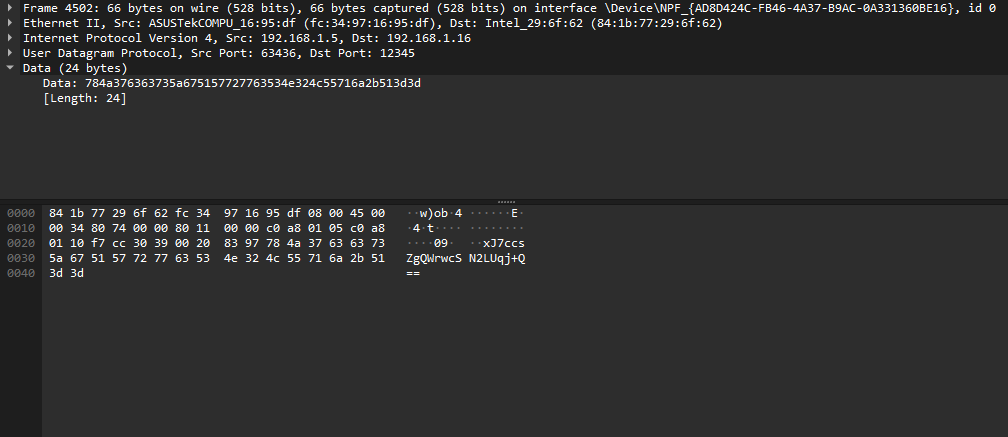
\includegraphics[width=1\linewidth]{Screenshot 2024-12-12 112958.png}
    \caption{Individual Text Package}
    \label{fig:enter-label}
\end{figure}

\newpage
\section{Audio Communication}
This java application, apart from text messaging, is also capable of real-time voice communication \textbf{(VoIP)}. This is also achieved using the \textbf{UDP Protocol}, and more specifically using a \textbf{44100 Hz} sampling rate, with a \textbf{16 bit} sampling size in a \textbf{stereo} channel.

The audio communication process is a bit more complicated compared to the text messaging implementation. Firstly, a separate thread is created for handling call requests in a separate \textbf{requests port}, "12347". This is done to notify the receiver of the call request, and give him the option of either rejecting, or accepting the call. If the call is rejected, using the same port, a rejected message is sent to the user initiating the call, notifying him the the call request was rejected. The snippets for the request-listening thread and the function to send these request messages are shown below:
\begin{lstlisting}[style=javastyle]
new Thread(() -> {
	byte[] buffer = new byte[1024];
	try (DatagramSocket requestsSocket = 
                        new DatagramSocket(
                            Integer.parseInt(requestsPort)))
    {
		while (true) {
			DatagramPacket packet = new DatagramPacket(
                                        buffer, buffer.length);
			requestsSocket.receive(packet);
			if (packet.getAddress().getHostAddress().equals(destIp))
            {
				String message = new String(
                                    packet.getData(), 0,
                                    packet.getLength());
				handleCallMessages(message);
			}
		}
	} catch (IOException e) {
		e.printStackTrace();
	}
}).start();
\end{lstlisting}


\begin{lstlisting}[style=javastyle]
private static void sendCallMessages(String message) {
	try {
		DatagramSocket socket = new DatagramSocket();
		InetAddress address = InetAddress.getByName(destIp);
		byte[] buffer = message.getBytes();
		DatagramPacket packet = new DatagramPacket(
                                    buffer, buffer.length, address,
                                    Integer.parseInt(requestsPort));
		socket.send(packet);
		socket.close();
	} catch (IOException e) {
		e.printStackTrace();
	}
}
\end{lstlisting}

\newpage
A function to handle all the request messages (for example "CALL\_REJECTED") is needed to ensure that the correct actions are taken depending on the message received. if the call is terminated by any of the users, an "end call" message will be sent to the other user, executing the \textbf{endCall()} function, necessary for closing any used sockets and speaker/ microphone in order to prevent data leaks. If the call is accepted, both users will execute the functions \textbf{startAudioCommunication()} for sending the audio data from the microphone, while in a separate thread, \textbf{startAudioReception()} for listening for packages in a separate thread and outputting their contents on a speaker. The snippets for all of these functions is shown below:
\begin{lstlisting}[style=javastyle]
private static void handleCallMessages(String message) {
	switch(message) {
		case "CALL_REQUEST":
			int response = JOptionPane.showConfirmDialog(
                           null, "Do you want to accept the call?", 
                           "Incoming call", JOptionPane.YES_NO_OPTION);
			if (response == JOptionPane.YES_OPTION) {
				sendCallMessages("CALL_ACCEPTED");
				startAudioCommunication();
				startAudioReception();
				callInProgress = true;
				callButton.setText("End");
			} else
				sendCallMessages("CALL_REJECTED");
			break;
		case "CALL_ACCEPTED":
			startAudioCommunication();
			startAudioReception();
			callInProgress = true;
			callButton.setText("End");
			break;
		case "CALL_REJECTED":
			textArea.append("Call rejected by the recipient" + newline);
			break;
		case "CALL_END":
			endCall();
			textArea.append("Call ended by the other user" + newline);
			break;
		default:
			break;
	}
}
\end{lstlisting}

\newpage
\begin{lstlisting}[style=javastyle]
private static void endCall() {
	callInProgress = false;
	if (voiceSenderSocket != null && !voiceSenderSocket.isClosed()) {
		voiceSenderSocket.close();
	}
	if (voiceReceiverSocket != null && !voiceReceiverSocket.isClosed())
    {
		voiceReceiverSocket.close();
	}
	if (microphone != null && microphone.isOpen()) {
		microphone.close();
	}
	if (speaker != null && speaker.isOpen()) {
		speaker.close();
	}
	callButton.setText("Call");
}
\end{lstlisting}

\begin{lstlisting}[style=javastyle]
public static void startAudioCommunication() {
	new Thread(() -> {
		try {
			// Start capturing and sending audio data
			AudioFormat format = new AudioFormat(44100,16, 2,
                                                 true, true);
			DataLine.Info info = new DataLine.Info(
                                        TargetDataLine.class, format);
			microphone = (TargetDataLine) AudioSystem.getLine(info);
			microphone.open(format);
			microphone.start();

			byte[] buffer = new byte[1024];
			voiceSenderSocket = new DatagramSocket();
			InetAddress address = InetAddress.getByName(destIp);

			while (callInProgress) {
				int bytesRead = microphone.read(buffer, 0,
                                                buffer.length);
				DatagramPacket packet=new 
                                      DatagramPacket(buffer, bytesRead,
                                                     address,
                                                     Integer.parseInt(
                                                     voicePort));
				voiceSenderSocket.send(packet);
			}
		} catch (IOException | LineUnavailableException ex) {
			ex.printStackTrace();
		} finally {
			if(voiceSenderSocket!=null && !voiceSenderSocket.isClosed())
            {
				voiceSenderSocket.close();
			}
			if(microphone != null && microphone.isOpen()) {
				microphone.close();
			}
		}
	}).start();
}
\end{lstlisting}

\newpage
\begin{lstlisting}[style=javastyle]
public static void startAudioReception() {
	new Thread(() -> {
		try {
			// Start receiving and playing audio data
			AudioFormat format = new AudioFormat(44100, 16, 2,
                                                 true, true);
			DataLine.Info info = new DataLine.Info(
                                     SourceDataLine.class, format);
			speaker = (SourceDataLine) AudioSystem.getLine(info);
			speaker.open(format);
			speaker.start();

			voiceReceiverSocket = new DatagramSocket(Integer.parseInt(
                                                     voicePort));
			byte[] buffer = new byte[1024];

			while (callInProgress) {
				DatagramPacket packet=new DatagramPacket(buffer,
                                                         buffer.length);
				voiceReceiverSocket.receive(packet);
				speaker.write(packet.getData(), 0, packet.getLength());
			}
		} catch (IOException | LineUnavailableException ex) {
			ex.printStackTrace();
		} finally {
			if (voiceReceiverSocket!=null && 
                !voiceReceiverSocket.isClosed())
            {
				voiceReceiverSocket.close();
			}
			if (speaker != null && speaker.isOpen()) {
				speaker.close();
			}
		}
	}).start();
}
\end{lstlisting}
\newpage
Below, we see again a \textbf{Wireshark} window, showing all the packages being sent for the call implementation, as well as a window showing the contents of a specific packet with its network headers and payload.

\begin{figure}[h!]
    \centering
    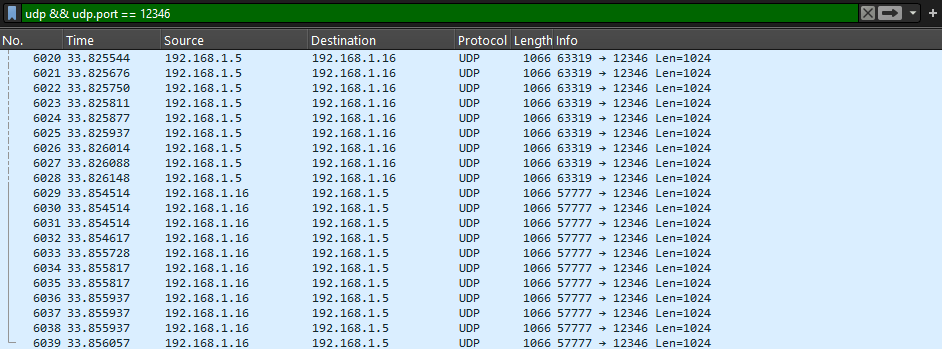
\includegraphics[width=1\linewidth]{Screenshot 2024-12-12 115616.png}
    \caption{Voice Packages List}
    \label{fig:enter-label}
\end{figure}

\begin{figure}[h!]
    \centering
    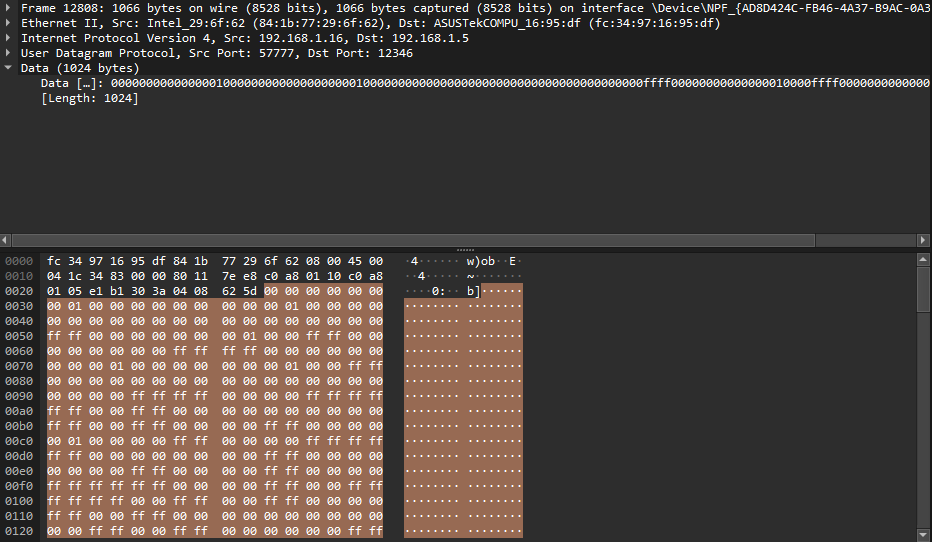
\includegraphics[width=1\linewidth]{Screenshot 2024-12-12 115653.png}
    \caption{Individual Voice Packet}
    \label{fig:enter-label}
\end{figure}

\newpage
We can also see any requests being sent on the requests port \textbf{12347} that handles call requests, rejections, and terminations as shown before:

\begin{figure}[h!]
    \centering
    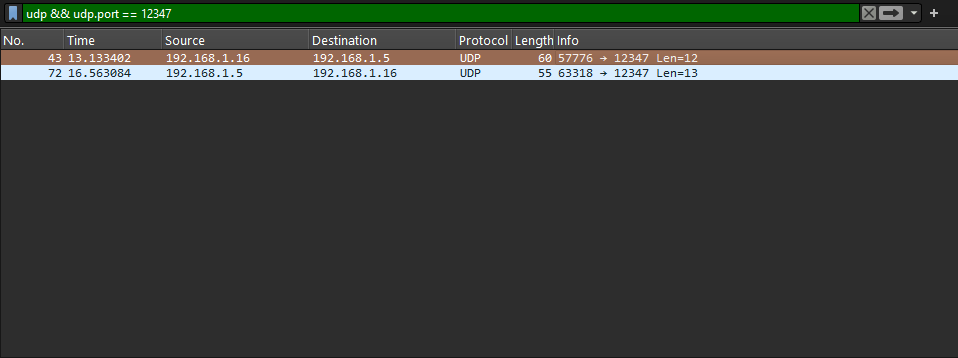
\includegraphics[width=1\linewidth]{Screenshot 2024-12-12 120132.png}
    \caption{Requests Packages List}
    \label{fig:enter-label}
\end{figure}

\begin{figure}[h!]
    \centering
    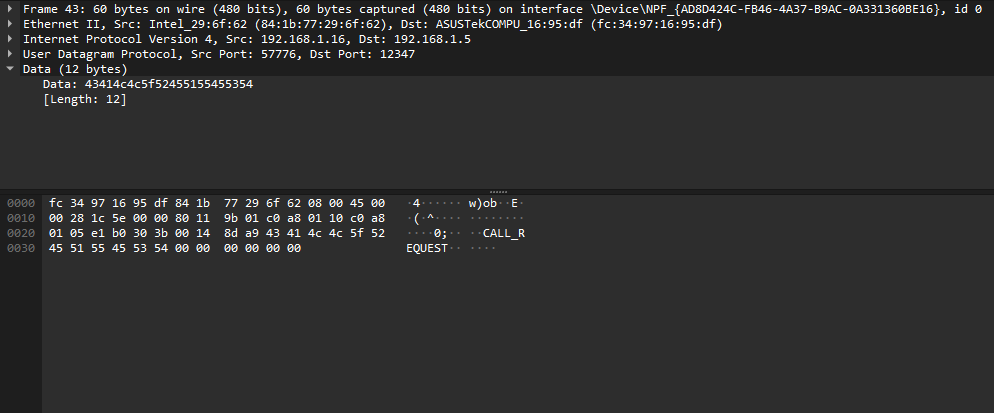
\includegraphics[width=1\linewidth]{Screenshot 2024-12-12 120151.png}
    \caption{Individual Request Packet}
    \label{fig:enter-label}
\end{figure}

\chapter{Tools Used}
The tools used for this implementation are:
\begin{itemize}
    \item The Java Programming Language.
    \item The \textbf{java.net} library for networking, as well as the \textbf{javax.sound} library for audio capture and playback.
    \item The \textbf{javax.crypto} library for encryption and decryption of the packages.
    \item Maven for build automation and project management for Java projects.
    \item GitHub for version control.
\end{itemize}

\end{document}